\documentclass[a4paper,10pt]{article}
\usepackage{graphicx}
\usepackage{enumitem}
\usepackage{amsmath}
\usepackage{listings}
\usepackage[usenames,dvipsnames]{color}
\usepackage{bbm}
\usepackage{amsfonts}
\usepackage{hyperref}
\usepackage{multicol}
\usepackage{caption}
\usepackage{xcolor}
\hypersetup{
    colorlinks,
    linkcolor={red!50!black},
    citecolor={blue!50!black},
    urlcolor={blue!80!black}
}
\newcommand{\cfbox}[2]{%
    \colorlet{currentcolor}{.}%
    {\color{#1}%
    \fbox{\color{currentcolor}#2}}%
}
\usepackage[thinlines]{easytable}
\usepackage{url}
\usepackage{relsize}
\renewcommand*{\UrlFont}{\ttfamily\smaller\relax}
\newcommand\fnurl[2]{%
  \href{#1}{#2}\footnote{\url{#1}}%
}
%%%%%%%%%%%%%%%%%%%%%%%%%%%%%%%%%%%%%%%%%%%%%%%%%%%%%%%%%%%%%%%%%%%%%%%%%%%%%%%%%%%%%%%%%%%
% MATLAB code listing
%
% This is the color used for MATLAB comments below
\definecolor{MyDarkGreen}{rgb}{0.0,0.4,0.0}
 
% For faster processing, load Matlab syntax for listings
\lstloadlanguages{Matlab}%
\lstset{language=Matlab, % Use MATLAB
frame=single, % Single frame around code
basicstyle=\tiny\ttfamily, % Use small true type font
keywordstyle=[1]\color{Blue}\bfseries, % MATLAB functions bold and blue
keywordstyle=[2]\color{Purple}, % MATLAB function arguments purple
keywordstyle=[3]\color{Blue}\underbar, % User functions underlined and blue
identifierstyle=, % Nothing special about identifiers
% Comments small dark green courier
commentstyle=\usefont{T1}{pcr}{m}{sl}\color{MyDarkGreen}\small,
stringstyle=\color{Purple}, % Strings are purple
showstringspaces=false, % Don't put marks in string spaces
tabsize=5, % 5 spaces per tab
%
%%% Put standard MATLAB functions not included in the default
%%% language here
morekeywords={xlim,ylim,var,alpha,factorial,poissrnd,normpdf,normcdf},
%
%%% Put MATLAB function parameters here
morekeywords=[2]{on, off, interp},
%
%%% Put user defined functions here
morekeywords=[3]{FindESS, homework_example},
%
morecomment=[l][\color{Blue}]{...}, % Line continuation (...) like blue comment
numbers=left, % Line numbers on left
firstnumber=1, % Line numbers start with line 1
numberstyle=\tiny\color{Blue}, % Line numbers are blue
stepnumber=5 % Line numbers go in steps of 5
}

\usepackage{xspace}
\newcommand*{\eg}{e.g.\@\xspace}
\newcommand*{\ie}{i.e.\@\xspace}

\makeatletter
\newcommand*{\etc}{%
    \@ifnextchar{.}%
        {etc}%
        {etc.\@\xspace}%
}
\makeatother
%%%%%%%%%%%%%%%%%%%%%%%%%%%%%%%%%%%%%%%%%%%%%%%%%%%%%%%%%%%%%%%5

\newcommand\scalemath[2]{\scalebox{#1}{\mbox{\ensuremath{\displaystyle #2}}}}


%opening
\title{Automatic Applicator\\System Conception}
\author{Munzir Zafar}

\begin{document}

\maketitle

\section{Introduction}

The purpose of this document is to thoroughly consider various solutions that can be used to solve the 
automatic painting problem meeting the specifications laid out in the earlier document. We firstly consider
why a robotic arm is more suitable in comparison to hard automation. Then we begin the process of 
coming up with an optimal design for the robotic arm. Among the decisions to be taken are:
\begin{enumerate}
 \item Should the base-link of the robot be on the floor of the painting area or on the roof/wall of the spraying booth?
 \item What are the alternatives of spraying guns that we will use? What are the sizes, weights and costs in each alternative being considered?
 \item What topology of the robot is optimal? 
 \item What are the optimal link-lengths in the considered topology?
 \item What kind of motors, and what ratings of the motors should be installed? Available alternatives with regards to sizes, weights and costs?
 \item What kind of gear-boxes should we use? What gear ratios should we use? What are the available alternatives? Their sizes, weights and costs?
 \item What options we have with regard to Motor Drives? Which is the best alternative?
 \item How do we implement position sensing? What is the best alternative?
 \item How does it all come together? The material, shape, size, and manufacturing process to be used for the mechanical links?
 \item What kind of controller or central processing system is to be used?
 \item Which power supply is to be used?
 \item What topology of electrical system for power, control and inter-system communication is to be used? 
 \item What is the user-interface going to look like?
\end{enumerate}

\section{Design Strategy}
Those are a lot of questions and we see that we have a large set of design variables to choose from. We also note
that there is hardly a design variable that is not dependent on other design varibles. For example, choosing a different
spraying gun would mean a different set of motors to be installed and thus a different set of gear-boxes. Finding the optimal solution
is a complex problem and we will benefit from optimization techniques in order to optimize the design variables. We will use the
following strategy in our design:
\begin{enumerate}
 \item We will not make an early decision with regards to whether to use the floor or the roof/wall of the chamber for placing the base-link. We will instead carry 
 out thorough analysis for both alternatives separately. The optimal design for both analysis will be evaluated. Then the two optimal solutions will be compared
 with each other and the pros and cons will be weighed to come up with a final decision with regards to the base link.
 \item We will research the range of spraying guns available so that we come up with the range of payloads to be lifted by our robot. A decision will not be taken
 as yet. Instead an optimal solution for each payload will be determined. We expect the optimal solution to remain the same for specific ranges of the payload.
 Once we have a clear idea as to how our decision of spraying gun weights are affecting the optimal robot design, we will be in a better position to select one
 spraying gun among many.
 \item The topology, link-lengths, motor-ratings and gear-boxes will be simultaneously evaluated using an iterative optimization algorithm. The objective of optimization
 is to minimize the cost while satisfying the specifications laid out in the \emph{Requirement Specifications} document. Two sets of optimal solution
 will be delivered at this stage, one for base-on-ground and the other for base-in-chamber. Each set of optimal solutions will contain optimal solutions for 
 each payload (spraying gun alternative) under consideration. A decision for the spraying gun will be taken at this stage so that we will have one optimal 
 solution from each set. The two solutions will then be weighed and a decision will be taken for the base-link placement.
 \item Motor-drives, sensors, links, processor, power-supply, electrical system and user-interface will subsequently be decided based on the optimal designs 
 carried out in the earlier steps. This is because it is assumed that these decisions can be taken independently without affecting the optimality of the solution we come up with
 out in the previous step.
\end{enumerate}
The above process will be done twice. Firstly, only for base-on-chamber-wall with a preliminary estimate of avaliable alternatives for spraying guns, motors and gear-boxes and secondly, with a more thorough
research on these alternatives for both base-on-ground and base-in-chamber. The focus in the former stage will be on developing the optimization procedure with a given set of design variables. Once the optimization
procedure is understood, then it will be repeated with more complete information of the available alternatives. The purpose is avoid getting bogged down by the sheer range of available options for these parts so that we stay focussed on the conceptualization of the design.


\section{Hard Automation Versus Robotic Arm}

\section{Designing the Robot Arm}

\subsection{Formulating the Optimization Problem}
\subsubsection{Design Variables}
Regardless of whether the base is on ground or it is on the roof/wall and assuming a specific pay load, the problem at hand
is that of optimization where we are trying to take optimum decisions for the the following five variables:
\begin{itemize}
  \item Location of the base link
  \item Configuration of the actuators
  \item Link lengths
  \item Motors
  \item Gearboxes
\end{itemize}

\subsubsection{Range}
Before we begin optimization, we need to know the available options we have for the five variables that we are trying to choose the optimum from. 
\begin{enumerate}
  \item Base link location: All locations that will allow the existence of a robot that can access the workspace with six or less actuators are included in the range of available options.
  \item Configuration of the actuators: In each of the base link location, any actuator configuration that can access the workspace with six or less actuators are included in the range of available options.
  \item Link Lengths: For each actuator configuration the lengths of the links that can access the workspace with six or less actuators are included in the range of available options.
  \item Motors: All motors available on the market.
  \item Gearboxes: All gearboxes available on the market.
\end{enumerate}

\subsubsection{Objective}
What we are trying to optimize is the total cost of production of the design.

\subsubsection{Constraints}
The \emph{Requirement Specifications} of the robot are the constraints that the robot needs to satisfy.

\subsection{Range of Base-Link Location}
We need to determine all the possible locations at which the base link can be placed while still reaching
the workspace with five or six DOFs. We are assuming that feasible base-locations form a continuous set in the world-space, with certain boundaries. For example, feasible space would
be bounded by how close it can be to the workspace and yet reach all the task locations. The problem will become relatively simpler if we reduce it to 3 DOF problem. That is, we design only a 3 DOF robot
that can reach any location in the workspace without worrying about the orientation of the end-effector. The inclusion of orientation may result in
further shrinkage of the feasible space but we surmise that it will not be too different, even though the complexity of the problem is significantly reduced by changing it to 3DOF.
Our approach will be of searching this boundary. We will search through the space using random base-locations. Each location will be admitted to the feasible space if there exists a configuration that can reach all points in the task space. If the point was not feasible we will move further away from the workspace in our next iteration, otherwise we will move closer to the workspace. This procedure will be performed along a several pre-selected lines that sufficiently cover the entire neighborhood of the workspace as shown in figure \ref{fig:baseLinkSearchLines}. Note also that we will limit the search space to the neihbourhood of only a quarter of the top surface, and its adjacent quarters on the side surfaces. This is done because of symmetry of the workspace. The feasible space obtained for the selected neighborhood can be easily mirrored to other neighborhoods.

\begin{figure}[h]
\centering \frame{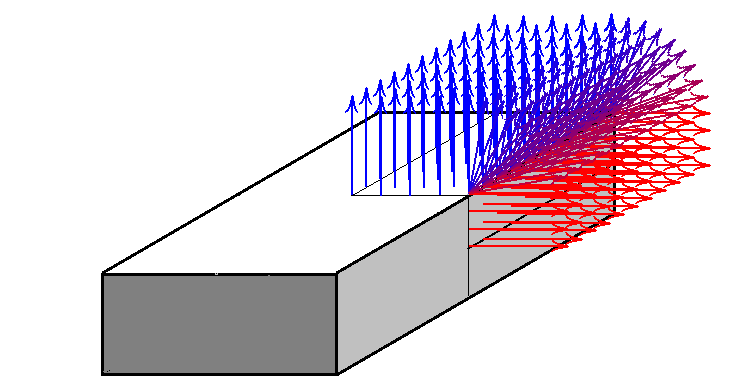
\includegraphics[width=0.8\columnwidth]{Figures/baseLinkSearchLines.png}}
\caption{The lines along which we will search the boundary of the feasible space}
\label{fig:baseLinkSearchLines} 
\end{figure}

For a 3R chain, a general forward and reverse kinematic model can be derived using DH parameters. For a given set of task positions that give sufficient coverage of the workspace, we will formulate a mathematical relationship that can determine for us the range of DH paramters that will solve the problem. If we are able to find that mathematical formulation, then we will use this relationship to check existence of a solution on each search line described above, with the aim of searching for the feasibility boundary. If such a mathematical formulation does not exist then we will have to look into simulated annealing and figure out how to implement it.


\subsection{Developing and Understanding Optimization Procedure Using Preliminary Estimates on the Range of Available Design Options}

\subsection{Listing Down the Alternatives}

\subsubsection{Specifications for Base-Link Placement Alternatives}

\subsubsection{Alternatives for Spray Guns}
\tiny
\begin{multicols}{4}
\begin{enumerate}
  \item \fnurl{http://www.sedco.co.uk/pages/automatic_sprayguns.htm}{Sedco}
  \item \fnurl{http://www.tradeindia.com/manufacturers/painting-robots.html}{Trade India}
  \item \fnurl{http://www.takubo.co.jp/e/product/gun/spraygun.html}{Takubo}
  \item \fnurl{http://schuberts.co.uk/products/finishing-systems/robotic-spray-systems-2/}{Schuberts}
  \item \fnurl{http://spray-direct.co.uk/products-pla/page/2/}{Spray Direct}
  \item \fnurl{http://drstienecker.com/tech-332/14-end-effectors-and-applications/}{Dr. Stienecker}
  \item \fnurl{http://www.polyurea.com/spps/ahpg.cfm?spgid=37}{Polyurea}
  \item \fnurl{https://www.google.com.pk/url?sa=t&rct=j&q=&esrc=s&source=web&cd=121&cad=rja&uact=8&ved=0CBkQFjAAOHhqFQoTCP6-4tGE4sgCFYM0lAodBs4EZQ&url=http\%3A\%2F\%2Fwww.dete.de\%2Fletoeltesek.html\%3Ffile\%3Dfiles\%2Fdete\%2Fcontent\%2Fdownloads\%2FLackierpistolen\%2520und\%2520Zubehoer\%2520Prospekt\%2520EN.pdf&usg=AFQjCNHxoVyBPJn_rLP4LW79k0Ze8oHGyg&sig2=UZV_6pMTehIajOxfHjEMeg}{Dete}
  \item \fnurl{http://sprayworksequipment.com/spray-foam-products/spray-foam-robotics-spraybot/}{Sprayworks Equipment}
  \item \fnurl{http://www.parker-eng.co.jp/en/product/l-plant/robot/}{Parker Eng}
  \item \fnurl{http://www.directindustry.com/prod/sames-technologies/product-13892-415762.html}{Direct Industry}
  \item \fnurl{http://www.yamaguchigiken.co.jp/english/seihin/ichiran/7.html}{Yama Guchi Giken}
  \item \fnurl{http://www.devilbiss.com/products/spray-guns/automatic-spray-guns/hvlp/compact-automatic-i-hvlp-spray-gun\#LiveTabsContent36831760-lt}{Devilbiss}
  \item \fnurl{http://www.autotecno.com/pdf/automatic-sprayguns.pdf}{Autotecno}
  \item \fnurl{http://www.reiter-oft.de/en/painting-systems/atomizer-technology/air-atomizing-spray-guns.html}{Reiter Oft}
  \item \fnurl{http://www.anest-iwata.co.jp/english/paint/spraygun/ta2vfs0000004gmi.html}{Anest Iwata}
  \item \fnurl{http://supersonicspray.com/en/products/robotics-spray-guns}{Supersonic Spray}
  \item \fnurl{https://www.sata.com/index.php?id=automatic&L=11}{Sata}
\end{enumerate}
\end{multicols}

\subsubsection{Motor Alternatives}

\subsubsection{Gear-Box Alternatives}

\subsection{Design Optimization for Dependent Design Variables}

\subsection{Optimizing Indepedent Design Decisions}
\subsubsection{Motor Drives}

\subsubsection{Position Sensing}

\subsubsection{Mechanical Links}

\subsubsection{Controller}

\subsubsection{Power}

\subsubsection{Electrical System}

\subsubsection{User Interface}

\newpage
\begin{align}
 b\times(b\times X) &= b(b\cdot X)-X(b\cdot b) \nonumber \\
 b\times(X\times b) &= X(b\cdot b)-b(b\cdot X) \nonumber \\
\end{align}

\end{document}
